\section{Auswertung}
\label{sec:Auswertung}
\subsection{Messung im Niederdruckbereich bis 1 bar} % (fold)
\label{sub:Niederdruck_aus}


\begin{figure}
  \centering
  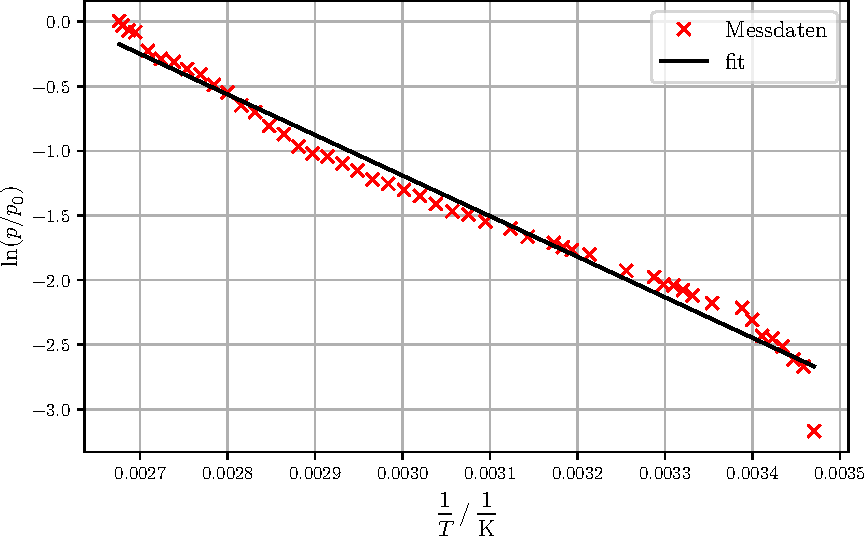
\includegraphics[scale=0.7]{build/plot1.pdf}
  \caption{Messwerte und Ausgleichsgerade im Niederdruckbereich bis 1 bar.}
  \label{fig:plot1}
\end{figure}

In \autoref{fig:plot1} ist das logarithmierte Verhältnis von $p$ und $p_0$ aufgetragen gegenüber dem Kehrwert der Temperatur.
Der Umgebungsdruck $p_0$ beträgt vor Beginn der Messung \qty{1024}{\milli\bar}. 
Zusätzlich ist eine lineare Ausgleichsgerade der Messwerte dargestellt. Die Parameter der Ausgleichsgerade
\begin{align*}
  a &= (-3139.31 ± 69.53) \si{\kelvin}\\
  b &= (8.23 ± 0.21),
\end{align*}
sowie die Fehler werden mit den Pythonmodulen Matplotlib \cite{matplotlib}, Scipy \cite{scipy} und Uncertainties \cite{uncertainties} berechnet.
Die dafür verwendeten Formeln sind in \autoref{sec:Fehlerrechnung} zu finden.

Durch Umstellen von \autoref{eqn:CC-Gl_2} und \autoref{eqn:lina} berechnet sich $L$ durch
\begin{align*}
  L&= -a R\\
\shortintertext{zu}
  L &= (2.61\pm 0.06)\cdot 10^4 \si{\joule\per\mol},
\shortintertext{wobei}
  R &=8.314
\end{align*}
die allgemeine Gaskonstante ist.
$L$ setzt sich zusammen aus der inneren Verdampfungswärme $L_i$, also der Energie die nötig ist um die molekularen Bindungskräfte zu überwinden und der
äußeren Verdampfungswärme $L_a$, also der Energie die nötig ist um das Volumen eines Mols im flüssigen Zustand auf das Volumen eines Mols im gasförmigen Zustand zu vergrößern.

Die äußere Verdampfungswärme bei $T=\qty{373}{\kelvin}$ wird durch 
\begin{align*}
  L_a&=R T
  \shortintertext{berechnet zu}
  L_a&= 3101.12 \si{\joule\per\mol}.
\end{align*}

Daher ergibt sich $L_i$ zu 
\begin{align*}
  L_i= (2.30 \pm 0.06)\cdot 10^4 \si{\joule\per\mol}.
\end{align*} 
Zur verbesserten Darstellung dieser Größe wird sie pro Molekül ausgedrückt und in $\si{\electronvolt}$ umgerechnet. Somit ergibt sich
\begin{align*}
  L_i = (2.30 \pm 0.06)\cdot 10^4 \si{\joule\per\mol} \mathbin{/} N_A = (0.24 \pm 0.01) \si{\electronvolt},
\end{align*}
wobei $N_A$ die Avogadro-Konstante ist.

\subsection{Messung im Hochdruckbereich von 1 bis 15 bar} % (fold)
\label{sub:Hochdruck_aus}


\begin{figure}
  \centering
  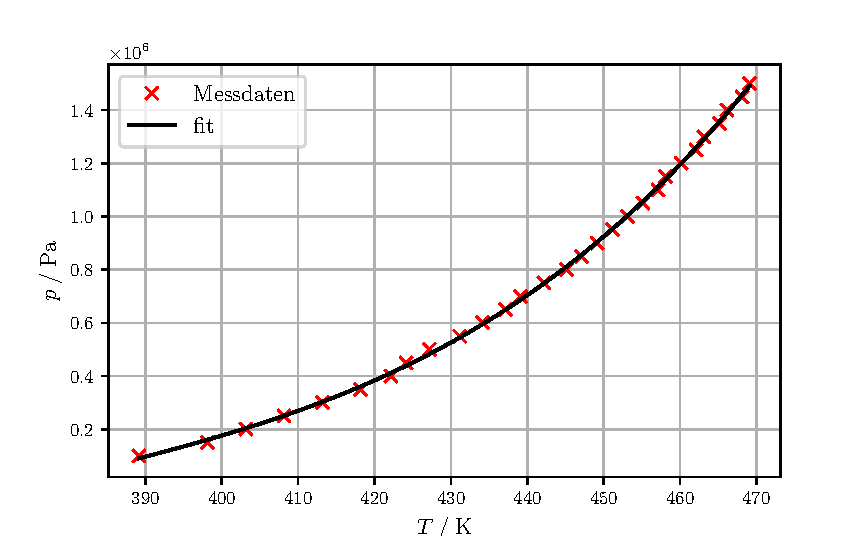
\includegraphics[scale=0.7]{build/plot2.pdf}
  \caption{Messwerte und Ausgleichsgerade im Hochdruckbereich von 1 bis 15 bar.}
  \label{fig:plot2}
\end{figure}
In \autoref{fig:plot2} sind die Messwerte für $p$ im Hochdruckbereich von $\qty{1}{\bar}$ bis $\qty{15}{\bar}$ gegenüber der Temperatur $T$ aufgetragen.
Zusätzlich wird auch hier eine Ausgleichsfunktion geplottet.
Die Funktion lautet 
\begin{align}
  p(T)= aT^3+bT^2+cT+d\label{eqn:polynom}
\end{align}
und ihre Parameter werden bestimmt zu
\begin{align*}
  a &= (1.20 ± 0.16) \si{\pascal\per\kelvin\tothe{3}}\\
  b &= (-1.37 ± 0.21)\cdot 10^3 \si{\pascal\per\kelvin\tothe{2}}\\
  c &= (5.30 ± 0.90)\cdot 10^5 \si{\pascal\per\kelvin}\\
  d &= (-6.90 ± 1.29)\cdot 10^7 \si{\pascal}.
\end{align*}

Zur Bestimmung von $L$ wird die Ableitung 
\begin{align}
 \frac{p(T)}{dT}= 3aT^2+2bT+c
\end{align}
gebildet.

\autoref{eqn:CC-Gl} wird nach $L$ umgeformt zu
\begin{align}
  L= T(V_D\,-\,V_F) \frac{dp}{dT}.
\end{align}
$V_F$ wird auch im Folgenden vernachlässigt. $V_D$ gehorcht im Hochdruckbereich nicht mehr der allgemeinen Gasgleichung \eqref{eqn:idGas}, sondern
wird näherungsweise durch
\begin{align}
    \left( p + \frac{A}{V^2} \right)  V = R  T
\shortintertext{mit} 
  A = \SI{0.9}{\joule\meter\cubed\per\mol\squared} \\
\shortintertext{zu}
V_{\text{D},\pm} = \frac{R T}{2  p} \pm \sqrt{\frac{R^2  T^2}{4  p^2} - \frac{A}{p}}
\end{align}
bestimmt.
Somit ergibt sich 
\begin{align}
  L= T \Biggl [ \frac{R  T}{2  p} \pm \sqrt{\frac{R^2  T^2}{4  p^2} - \frac{A}{p}} \Biggr ] \frac{dp}{dT}\label{eqn:L}
\end{align}
wobei für $p$ \autoref{eqn:polynom} eingesetzt wird.

In Graph \ref{fig:plot3} wird der positive Teil von \autoref{eqn:L} abhängig von $T$ dargestellt und in Graph \ref{fig:plot4} der negative Teil.

\begin{figure}[htbp]
  \begin{subfigure}{\textwidth}
  \centering
  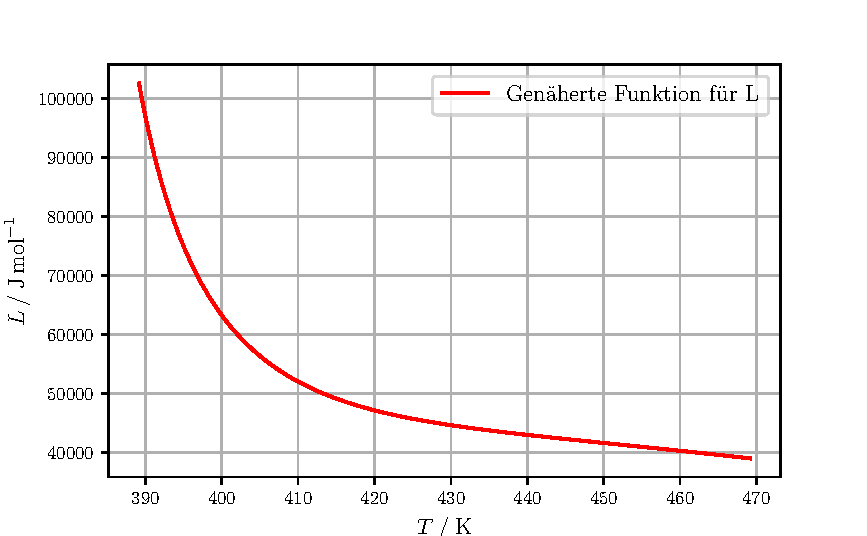
\includegraphics[scale=0.7]{build/plot3.pdf}
  \caption{positive Wurzel.}
  \label{fig:plot3}
\end{subfigure}
\begin{subfigure}{\textwidth}
  \centering
  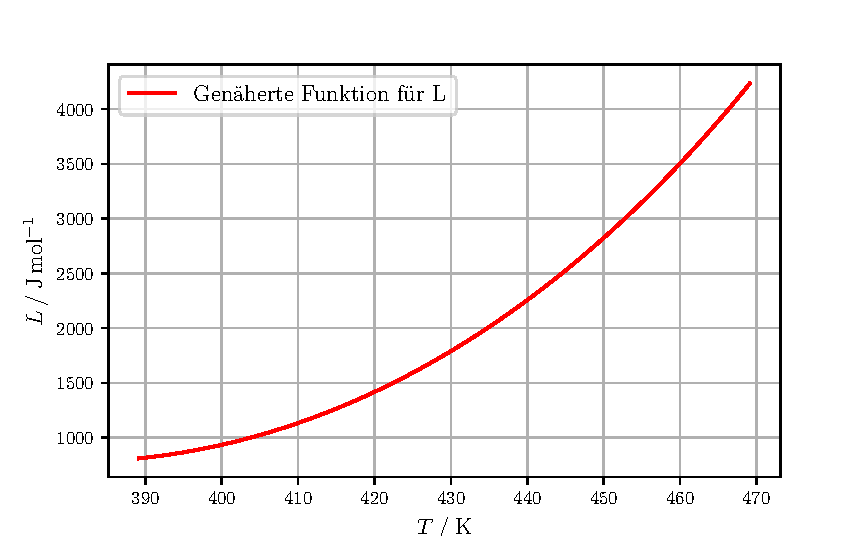
\includegraphics[scale=0.7]{build/plot4.pdf}
  \caption{negative Wurzel.}
  \label{fig:plot4}
\end{subfigure}
\caption{Graphen der Temperaturabhängigkeit von $L$.}
\end{figure}

